%CONFIGURACIÓN DEL DOCUMENTO Y HOJA

\documentclass[11pt,letterpaper]{article}
\setlength{\parindent}{0em}                  %DISTANCIA SANGRÍA
\setlength{\parskip}{0.5em}                  %DISTANCIA ENTRE PÁRRAFOS
\textwidth 6.5in
\textheight 9.in
\oddsidemargin 0in
\headheight 0in

%PAQUETES DEL TEMPLATE

\usepackage{fancybox}
\usepackage[utf8]{inputenc}
\usepackage{epsfig,graphicx}
\usepackage{multicol,pst-plot}
\usepackage{pstricks}
\usepackage{amsmath}
\usepackage{amsfonts}
\usepackage{amssymb}
\usepackage{eucal}
\usepackage[left=2cm,right=2cm,top=2cm,bottom=2cm]{geometry}
\usepackage{txfonts}
\usepackage[spanish]{babel}
\usepackage[colorlinks]{hyperref}
\usepackage{cancel}
\usepackage{caption}
\usepackage{float}
\usepackage{upgreek}
\usepackage{gensymb}
\usepackage{subfigure}
\usepackage{siunitx}
\usepackage{color}
\usepackage{tikz}
\usepackage{listings}
\usepackage{minted}
\usepackage{mdframed}
\usepackage[
backend=bibtex,
style=ieee,
sorting=none
]{biblatex}
\addbibresource{biblio.bib}
\usepackage{multicol}

%DEFINICIÓN DE COLORES EXTRAS

\definecolor{codegreen}{rgb}{0,0.6,0}
\definecolor{codegray}{rgb}{0.5,0.5,0.5}
\definecolor{backcolour}{rgb}{0.95,0.95,0.95}
\hypersetup{colorlinks=true,linkcolor=codegreen,citecolor=blue,filecolor=blue,urlcolor=magenta,}

%CONFIGURACIÓN DE LSTLISTINGS PARA CÓDIGOS

\lstset{ %
language=python,                % choose the language of the code
basicstyle=\footnotesize,       % the size of the fonts that are used for the code
numbers=left,                   % where to put the line-numbers
numberstyle=\footnotesize,      % the size of the fonts that are used for the line-numbers
stepnumber=1,                   % the step between two line-numbers. If it is 1 each line will be numbered
numbersep=5pt,                  % how far the line-numbers are from the code
backgroundcolor=\color{white},  % choose the background color. You must add \usepackage{color}
showspaces=false,               % show spaces adding particular underscores
showstringspaces=false,         % underline spaces within strings
showtabs=false,                 % show tabs within strings adding particular underscores
frame=single,                   % adds a frame around the code
tabsize=2,                      % sets default tabsize to 2 spaces
captionpos=b,                   % sets the caption-position to bottom
breaklines=true,                % sets automatic line breaking
breakatwhitespace=false,        % sets if automatic breaks should only happen at whitespace
escapeinside={\%*}{*)}          % if you want to add a comment within your code
}
\lstdefinestyle{mystyle}{
	backgroundcolor=\color{backcolour},
	commentstyle=\color{red},
	keywordstyle=\bfseries\color{magenta},
	numberstyle=\tiny\color{codegray},
	stringstyle=\color{codegreen},
	basicstyle=\footnotesize\ttfamily,
	identifierstyle=\color{blue},
	breakatwhitespace=false,
	breaklines=true,
	captionpos=b,
	keepspaces=true,
	numbers=left,
	numbersep=5pt,
	showspaces=false,
	showstringspaces=false,
	showtabs=false,
	tabsize=2
}

\lstset{style=mystyle}

%CONFIGURACIÓN DE MINTED PARA CÓDIGOS

\usemintedstyle{vs}

%DEFINICIÓN DE COMANDOS EXTRAS

\pagestyle{empty}
\newcommand{\units}[1]{\left[ #1 \right]}          %CORCHETES PARA UNIDADES
\newcommand{\abs}[1]{\left|#1\right|}              %OPERADOR VALOR ABSOLUTO INTEGRALES

%COMIENZA EL DOCUMENTO

\begin{document}

%CONFIGURACIÓN DEL ENCABEZADO

\usetikzlibrary{positioning}
\tikzset{every picture/.style={line width=0.75pt}}
\pagestyle{plain}
\begin{flushleft}
Ingeniería de la Salud \hfill Bioinformática\\
Escuela Técnica Superior de Ingeniería Informática\\
\underline{Universidad de Málaga}
\end{flushleft}

\begin{flushright}\vspace{-5mm}

\includegraphics[height=1.5cm]{escudo.jpg}
\end{flushright}

\begin{center}\vspace{-1cm}
\textbf{\large Práctica 3. Aproximación Diofántica}\\   %TITULO
Arrabalí Cañete, Carmen Lucía\\                         %NOMBRE
\end{center}
\rule{\linewidth}{0.1mm}

%DESDE AQUÍ SE ESCRIBE TODO EL CONTENIDO

\section{Introducción y objetivos}
En la teoría de números, el estudio de la aproximación diofántica se encarga de aproximar números reales por medio de números racionales.

El primer problema consistía en saber hasta qué punto un número real puede ser aproximado por números racionales. Para este problema, un número racional $\frac{p}{q}$ es una \textquotedblleft buena\textquotedblright\ aproximación de un número real $\alpha$ si el valor absoluto de la diferencia entre $\frac{p}{q}$ y $\alpha$ no puede disminuir si $\frac{p}{q}$ se sustituye por otro número racional con un denominador menor. Este problema se resolvió en el siglo XVIII mediante las fracciones continuas.

\subsection{Enunciado matemático del método}
Sea $x \in \mathbb{R}$ un número real y $\epsilon \in \mathbb{R}^+$ una pequeña constante positiva, se desea encontrar $p$ y $q$ $\in \mathbb{Z}$ tal que $\frac{p}{q}$  $\left |  x - \frac{p}{q} \right | < \epsilon $ y, además, $p$ y $q$ son números relativamente primos, por lo que $\frac{p}{q}$ está en términos mínimos.

Al haber infinitos números racionales $\frac{p}{q}$ que se pueden aproximar a $x$ dentro de una tolerancia $\epsilon$, se dice que la mejor aproximación diofántica $\frac{p}{q}$ es  $\left |  x - \frac{p}{q} \right | < \left |  x - \frac{p'}{q'} \right | $ teniendo en cuenta que para cada número racional $\frac{p'}{q'}$ diferente de $\frac{p}{q}$ debe cumplir que $0 < q' \leqslant q$.

\section{Configuración del equipo}
Se ha realizado la implementación en un equipo con un sistema operativo Windows 10 Home 64 bits, con un procesador Intel$($R$)$ Core $($TM$)$ i7-6500U CPU $@$ 2.50GHz 2.59 GHz $($4 CPUs$)$ y un disco SSD de 480GB y 12GB de RAM. La versión Java corresponde a la número 17.

\section{Implemetación}

En el primer método de la implementación, \textit{protected RationalNumber getMiddlePoint} de la clase \textit{MediantApproximation} (ver apartado ~\ref{ch:31}) se encarga de calcular el punto medio entre dos números racionales L y R. En este caso, se calcula como la suma de los numeradores de ambos números y la suma de los denominadores de los mismos. 

\begin{center}
	Dado que L $= \frac{a}{c}$ y R $= \frac{b}{d}$, la mediana de ambos corresponde a M $= \frac{a+b}{c+d}$
\end{center}

Por otro lado, se tiene el método \textit{protected RationalNumber \_approximate} de la clase \textit{BinarySearchDiophantineApproximator} (ver apartado~\ref{ch:32}) que se encarga de realizar una búsqueda binaria entre dos números racionales L y R. 


\subsection{Método \textit{protected RationalNumber getMiddlePoint} de la clase \textit{MediantApproximation}}\label{ch:31}

\begin{lstlisting}[language = java]
	protected RationalNumber getMiddlePoint(RationalNumber l, RationalNumber r) {
		RationalNumber M = new  RationalNumber(l.numerator() + r.numerator(), l.denominator() + r.denominator());
		return M;
	}
\end{lstlisting}


\subsection{Método \textit{protected RationalNumber \_approximate} de la clase \textit{BinarySearchDiophantineApproximator}} \label{ch:32}
\begin{lstlisting}[language = java]
	protected RationalNumber _approximate(double x, double epsilon) {
		RationalNumber L = zero, R = one;	// rational numbers that enclose x
		RationalNumber M;					// the middle-ish point (a rational number between L and R).
		double Mfp;							// floating-point value of the middle-ish point
		double diff;						// difference between the middle-ish point and |x|
		
		if (x < epsilon) { 					
			M = zero;						
		}else if (x > (1-epsilon)) {		
			M = one;
		}else {
			// Perform binary search between L and R. Use
			// method getMiddlePoint to obtain a rational
			// number in-between L and R.
			do {
				M = getMiddlePoint(L, R);
				Mfp = M.asDouble();
				diff = Math.abs(Mfp - x);
				if (M.asDouble() <= x) {
					L = M;
				} else {
					R = M;
				}
			} while (diff >= epsilon);
			
		}
		return M;
	}
	
\end{lstlisting}

\section{Resultados y Conclusiones}
Para poder analizar correctamente los resultados, el método main recibe en los argumentos de entrada, varios modos de ejecución entre los que se encuentra \textit{$-$r $<$max\_digits$>$ $<$max\_num$>$} el cual genera un archivo con $<$max\_num$>$ números aleatorios con una longitud $<$max\_digits$>$ y calcula las aproximaciones con distintos valores de tolerancia, desde 0.1 hasta 10$^{-16}$.

Al utilizar ese modo de ejecución, se genera un archivo con los diferentes tiempos de ejecución, el cual se llama  un archivo \textit{Mediant-Approximation-stats.txt}.

Por otro lado, entre los recursos aportados en el Campus Virtual se tiene un archivo llamado \textit{analyze.R} que contiene un script el cual se encarga de generar una gráfica haciendo uso del archivo .txt generado anteriormente con el modo de ejecución $-$r.

\begin{figure}[H]
	\centering
	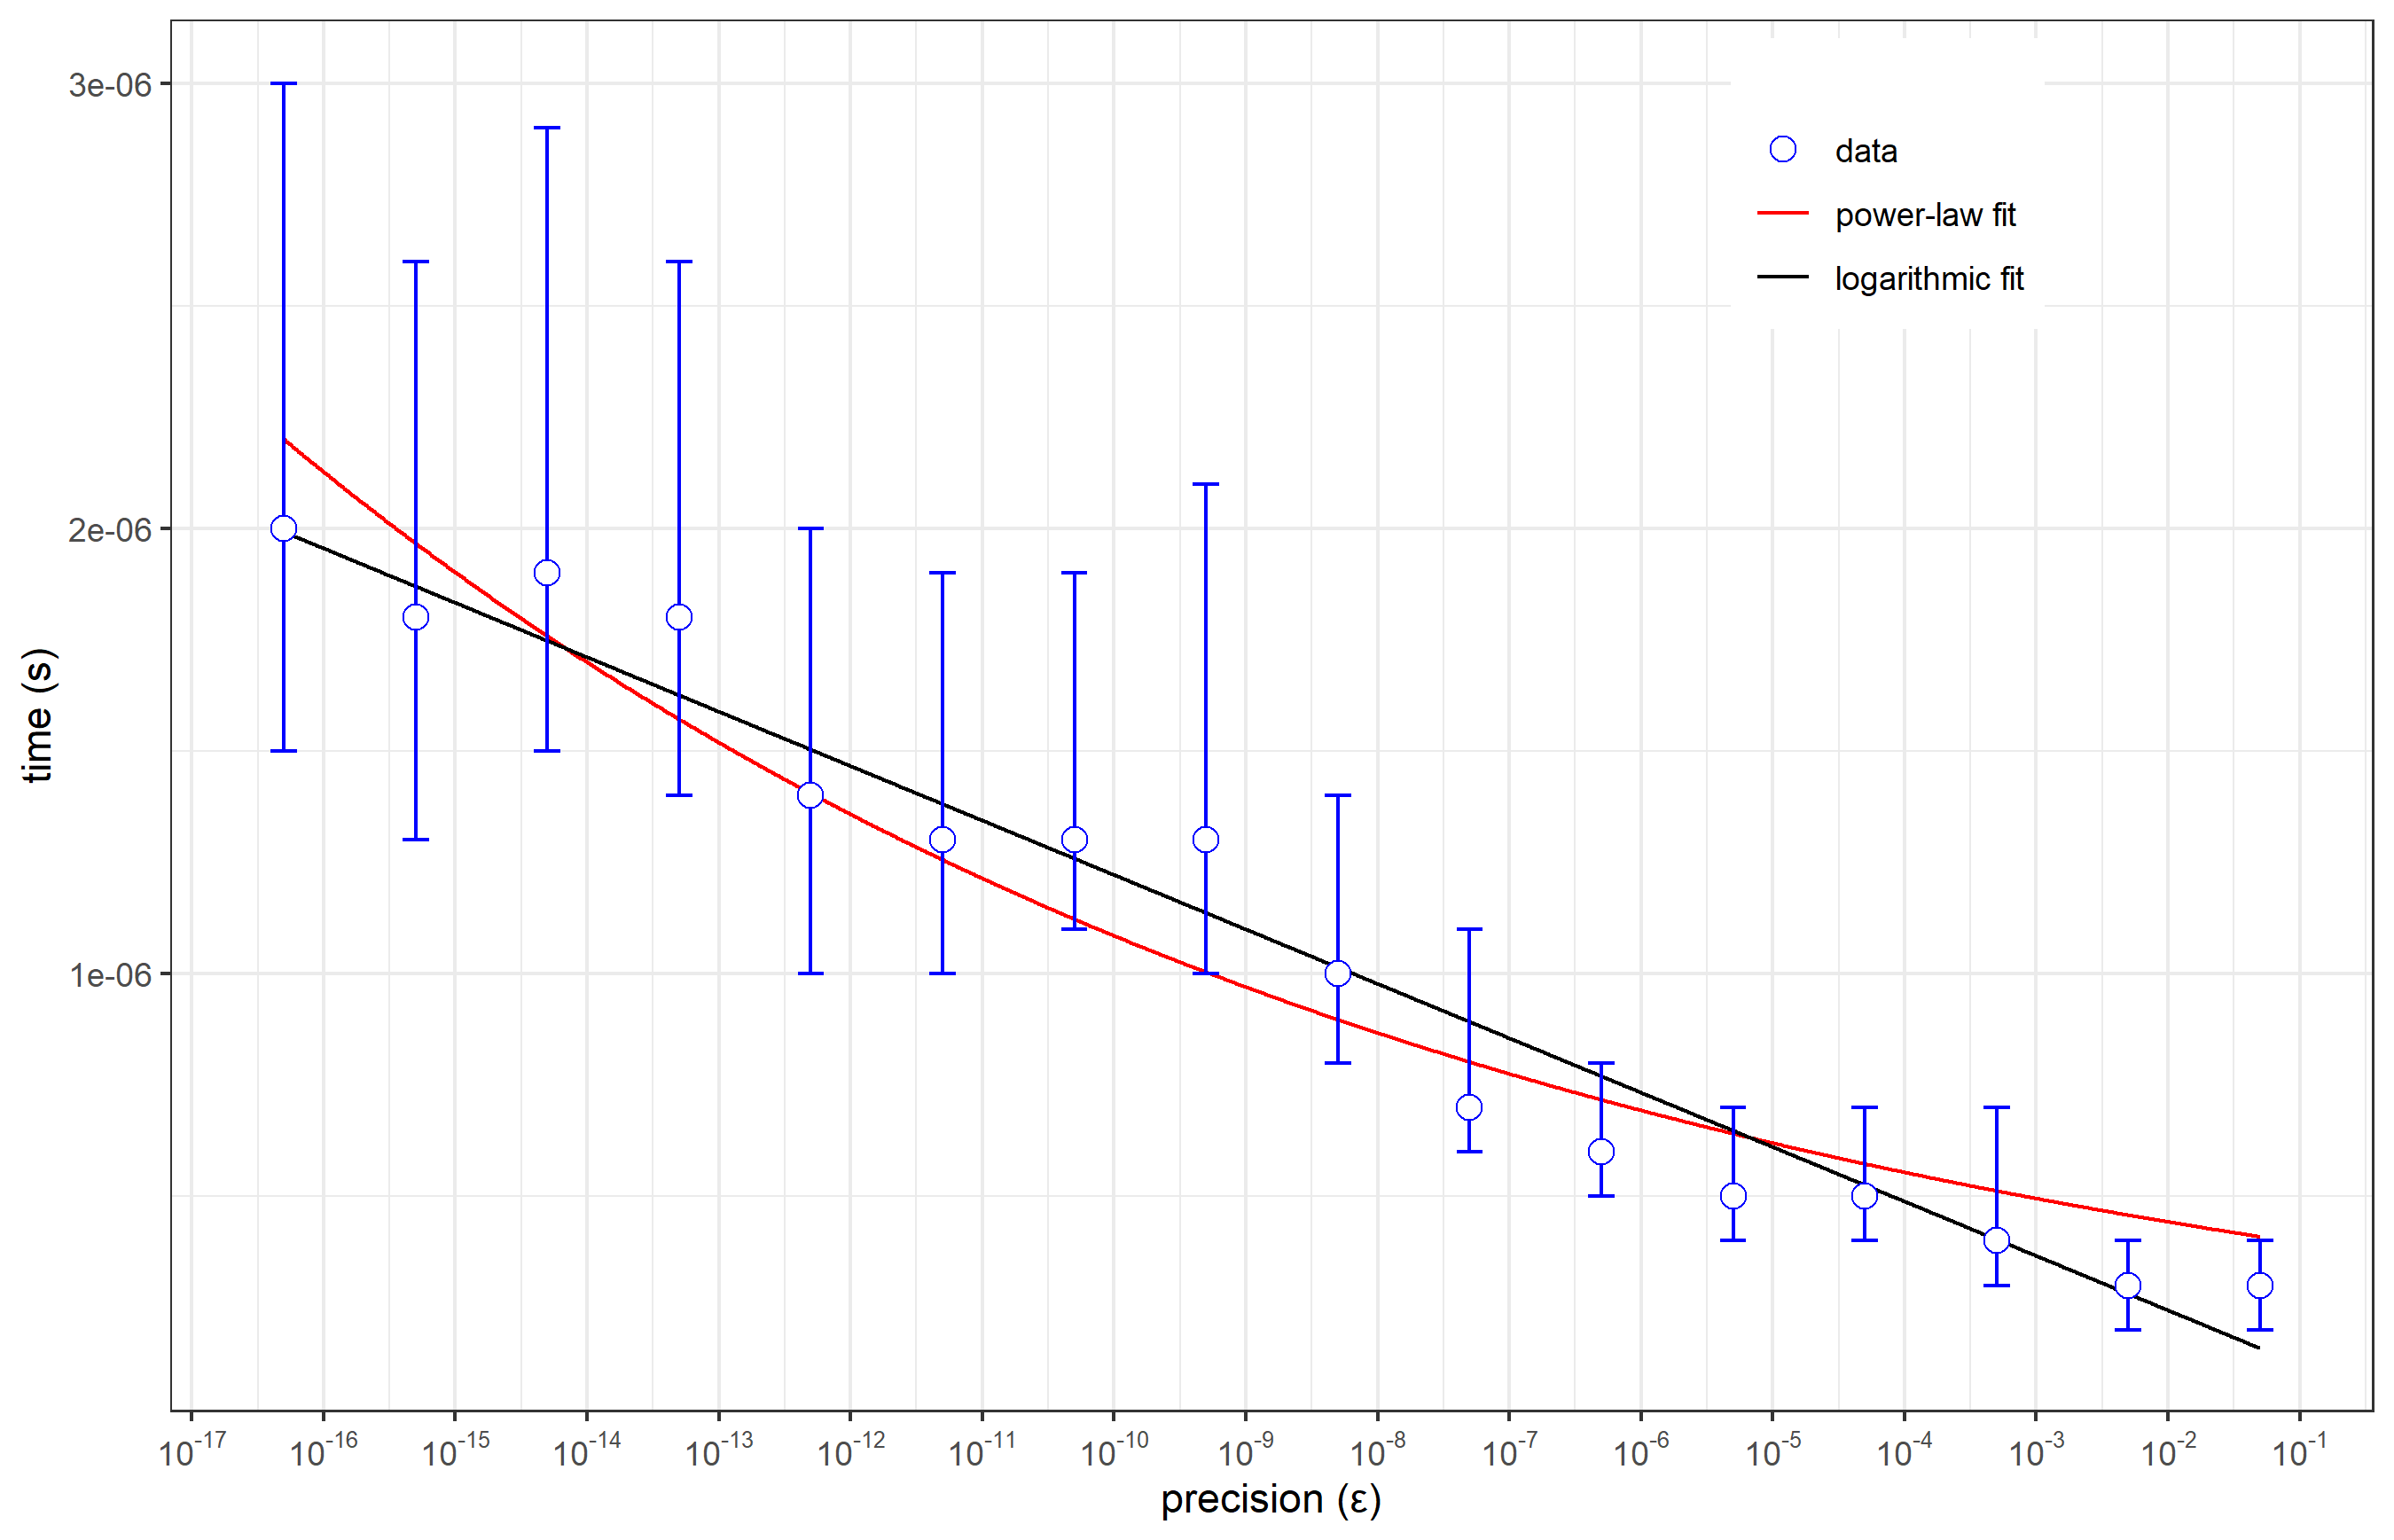
\includegraphics[width=0.65\textwidth]{mediant-approximation.png}
	\caption{Resultado de la ejecución del algoritmo con los parámetros utilizados.}
	\label{fig:grafico}
\end{figure}

Para poder obtener un buen conjunto de datos se han utilizado 50000 números con una longitud máxima de 16 caracteres. Como se puede observar en la figura~\ref{fig:grafico}, cuanta mayor sea la precisión con la que se quiere obtener la aproximación diofántica, el tiempo que tarda el algoritmo en obtener el resultado también es mayor. Se ajusta a la definición de la fórmula inicial, $\epsilon$ cuanto más pequeño es, menos diferencia tiene que haber con el número original.

\end{document}
